% !TEX root = main.tex
%%%%%%%%%%%%%%%%%%%%%%%%%%%%%%%%%%%%%%%%%%%%%%%%%%%%%%
\section{実験方法および結果}
%%%%%%%%%%%%%%%%%%%%%%%%%%%%%%%%%%%%%%%%%%%%%%%%%%%%%%
 実験装置を図の状態から90 [deg] 回転させ,初めに+方向に角速度を与えたときの角度推移を観測する.
実験を複数回行い,その平均値の角度推移をグラフにプロットする.また,同時に角速度の推移もプロットし,観測する.
なお,角速度データはノイズが多かったためカルマンフィルタを通し平滑化している.
\subsection{Duty比100\%・Duty比50\%による制御}
\subsubsection{実験方法}
 PWM信号のDuty比を,50\%と100\%にして実験を行う.


\subsubsection{実験結果}
 Duty比を50\%としたときの結果を図\ref{fig:duty50deg},図\ref{fig:duty50degpers}に,100\%としたときの結果を図\ref{fig:duty100deg},図\ref{fig:duty100degpers}に示す.
図に示すようにオーバーシュートが大きく,振動回数が2回となっている.
また,磁気トルカに触ると明らかに発熱していた.
発熱を抑えようとすれば整定時間が伸びる傾向にあった.

\begin{figure}[h]
	\centering
	\begin{minipage}{0.43\columnwidth}
	  \centering
	  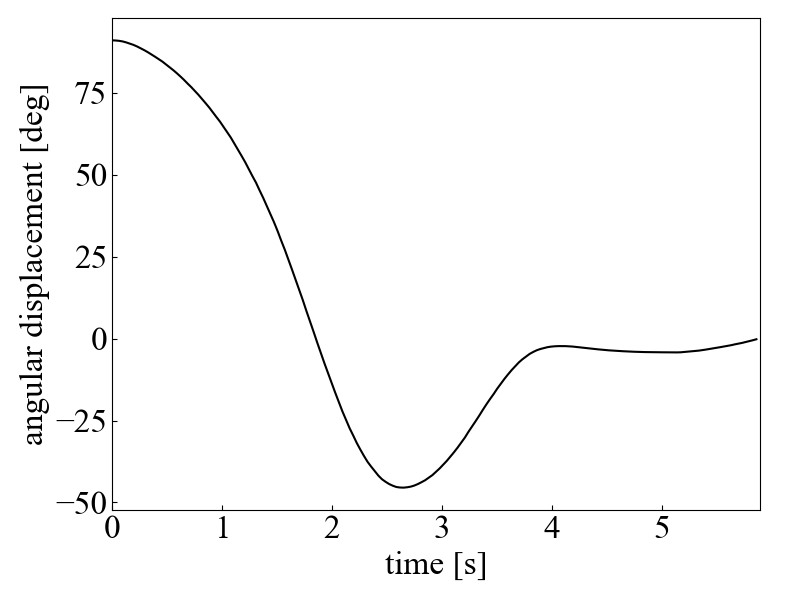
\includegraphics[width=\columnwidth]{./figure/duty50deg.png}
	  \caption{50\%としたときの角度推移}
	  \label{fig:duty50deg}
	\end{minipage}
	\hspace{5mm}
	\begin{minipage}{0.43\columnwidth}
	  \centering
	  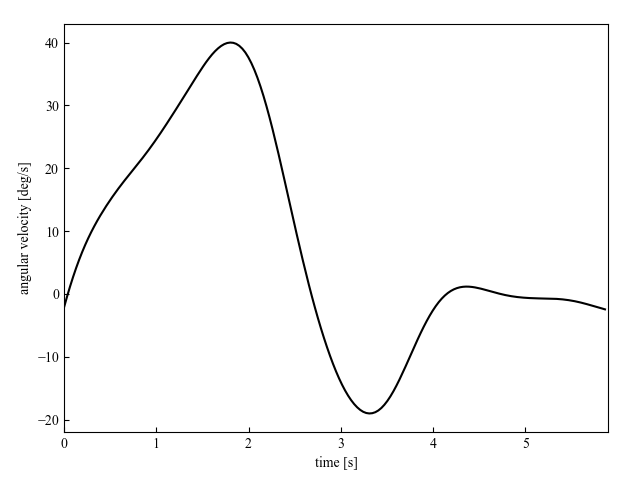
\includegraphics[width=\columnwidth]{./figure/duty50degpers.png}
	  \caption{50\%としたときの角速度推移}
	  \label{fig:duty50degpers}
	\end{minipage}
  \end{figure}

  \begin{figure}[h]
	\centering
	\begin{minipage}{0.43\columnwidth}
	  \centering
	  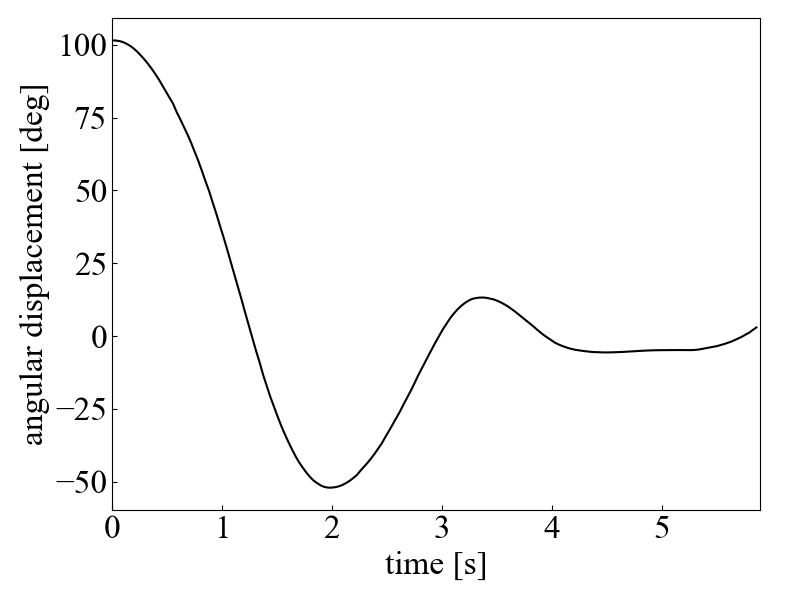
\includegraphics[width=\columnwidth]{./figure/duty100deg.png}
	  \caption{100\%としたときの角度推移}
	  \label{fig:duty100deg}
	\end{minipage}
	\hspace{5mm}
	\begin{minipage}{0.43\columnwidth}
	  \centering
	  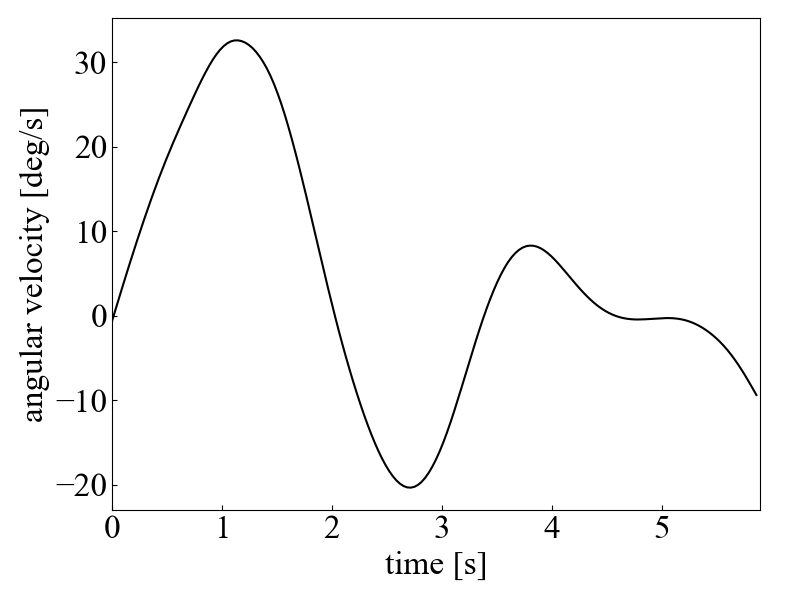
\includegraphics[width=\columnwidth]{./figure/duty100degpers.png}
	  \caption{100\%としたときの角速度推移}
	  \label{fig:duty100degpers}
	\end{minipage}
  \end{figure}

\newpage

\subsection{P制御}
\subsubsection{実験方法}
 Pコントローラを$I(t) = k_P |\theta(t)|$とし,

\subsubsection{実験結果}
 何度か実験を行って$k_P$を調整し,$k_P=0.05$としたときの結果を図\ref{fig:Pdeg},図\ref{fig:Pdegpers}に示す.
整定時間は3.8 s ,定常偏差は2.78 deg であった.

\begin{figure}[h]
	\centering
	\begin{minipage}{0.43\columnwidth}
	  \centering
	  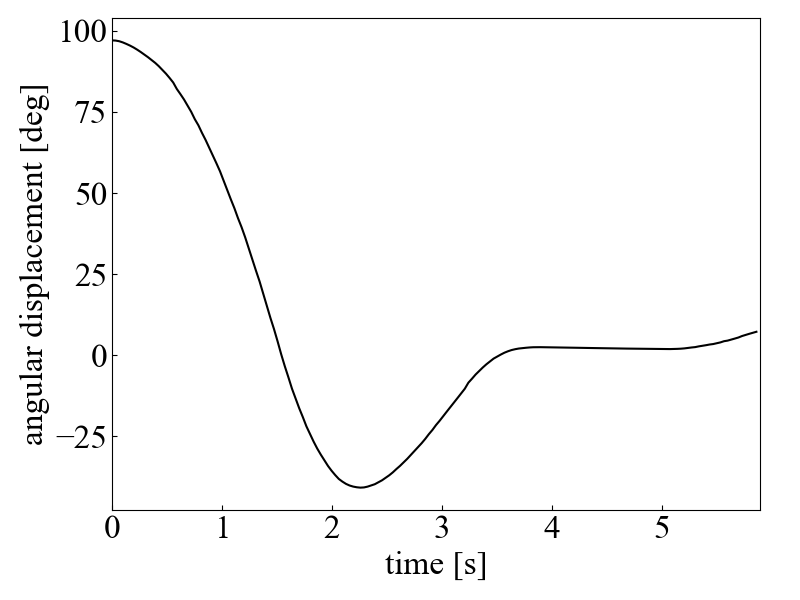
\includegraphics[width=\columnwidth]{./figure/Pdeg.png}
	  \caption{P制御の角度推移}
	  \label{fig:Pdeg}
	\end{minipage}
	\hspace{5mm}
	\begin{minipage}{0.43\columnwidth}
	  \centering
	  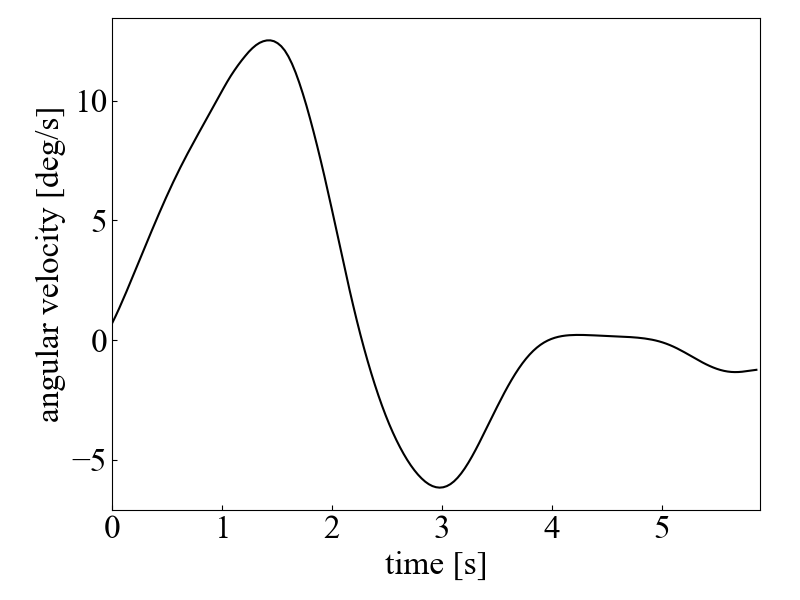
\includegraphics[width=\columnwidth]{./figure/Pdegpers.png}
	  \caption{P制御の角速度推移}
	  \label{fig:Pdegpers}
	\end{minipage}
  \end{figure}

\newpage

\subsection{PD制御}
\subsubsection{実験方法}
 Pコントローラを$I(t) = k_P |\theta(t)| + k_D|\frac{d\theta(t)}{dt}|$とする.
なお,$\frac{d\theta(t)}{dt}$は,プログラムの1ループ前の角度を$\theta_\mathrm{pre}(t)$とし,$\frac{d\theta(t)}{dt} = \theta(t)-\theta_\mathrm{pre}(t)$で近似する.
\subsubsection{実験結果}
 何度か実験を行ってゲインを調整し,$k_P=0.03$,$k_P=0.05$としたときの結果を図\ref{fig:PDdeg},図\ref{fig:PDdegpers}に示す.
整定時間は4.0 s ,定常偏差は-21.3 deg であった.
\begin{figure}[h]
	\centering
	\begin{minipage}{0.43\columnwidth}
	  \centering
	  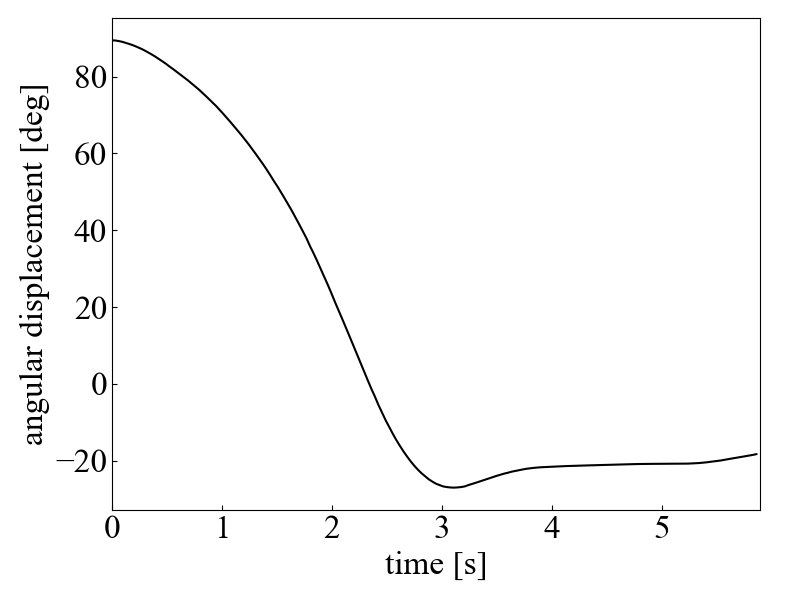
\includegraphics[width=\columnwidth]{./figure/PDdeg.png}
	  \caption{PD制御の角度推移}
	  \label{fig:PDdeg}
	\end{minipage}
	\hspace{5mm}
	\begin{minipage}{0.43\columnwidth}
	  \centering
	  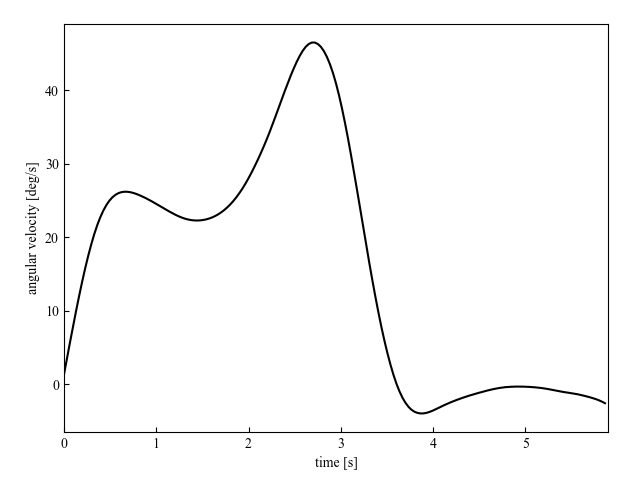
\includegraphics[width=\columnwidth]{./figure/PDdegpers.png}
	  \caption{PD制御の角速度推移}
	  \label{fig:PDdegpers}
	\end{minipage}
  \end{figure}

\subsection{B-dot制御則}
\subsubsection{実験方法}
 搭載する磁気トルカが1つであるので,目標磁気モーメントは$M=-k_bB_y\omega_z$である.
$|M|=nIS$より,コントローラを$I=\frac{-k_bB_y\omega_z}{nS}$として実験を行う.

\subsubsection{実験結果}
 $k_b=0.05$としたときの結果を図\ref{fig:kb5deg},図\ref{fig:kb5degpers}に示す.
整定時間は3.0 s ,定常偏差は-13.4 deg であった.

\begin{figure}[h]
	\centering
	\begin{minipage}{0.43\columnwidth}
	  \centering
	  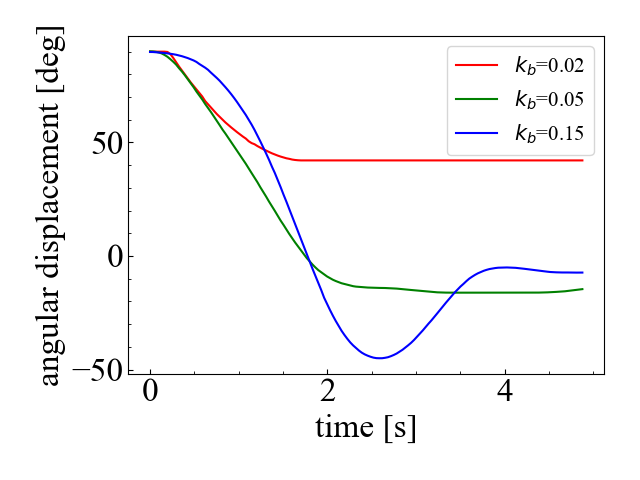
\includegraphics[width=\columnwidth]{./figure/kb5deg.png}
	  \caption{B-dot制御の角度推移}
	  \label{fig:kb5deg}
	\end{minipage}
	\hspace{5mm}
	\begin{minipage}{0.43\columnwidth}
	  \centering
	  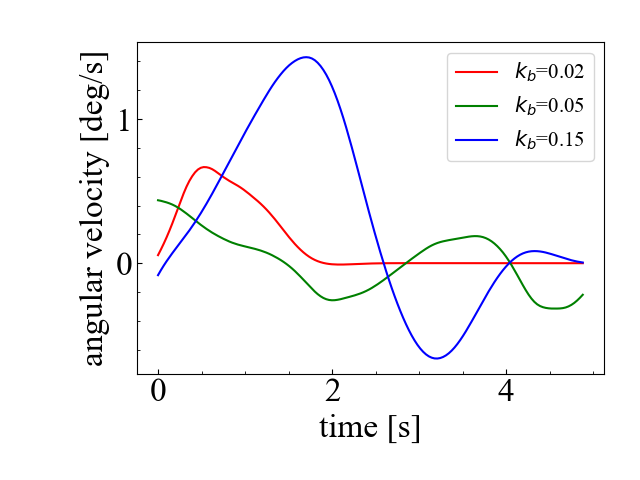
\includegraphics[width=\columnwidth]{./figure/kb5degpers.png}
	  \caption{B-dot制御の角速度推移}
	  \label{fig:kb5degpers}
	\end{minipage}
\end{figure}

\newpage

\subsection{クロスプロダクト則}
\subsubsection{実験方法}
 目標磁気モーメントが$M = \frac{K_x c_z + k_x \omega_z}{B_y}$であるので,
コントローラを$I=\frac{K_x c_z + k_x \omega_z}{nSB_y}$として実験を行う.

\subsubsection{実験結果}
 $K_x=0.04$,$k_x=0.03$としたときの結果を図\ref{fig:crossdeg},図\ref{fig:crossdegpers}に示す.
整定時間は3.8 s ,定常偏差は0.1 deg であった.

\begin{figure}[h]
	\centering
	\begin{minipage}{0.43\columnwidth}
	  \centering
	  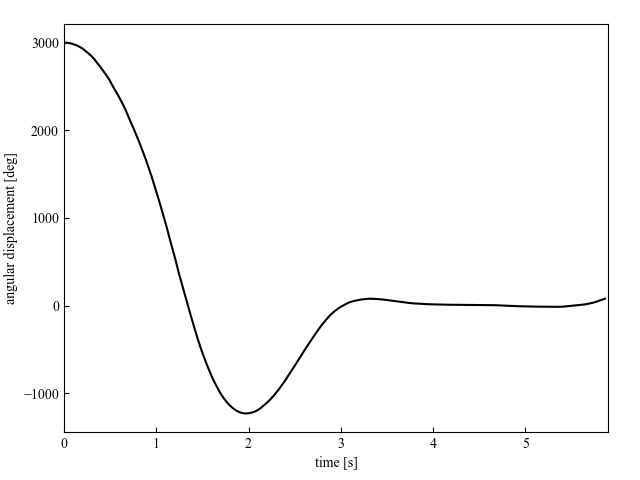
\includegraphics[width=\columnwidth]{./figure/crossdeg.png}
	  \caption{B-dot制御の角度推移}
	  \label{fig:crossdeg}
	\end{minipage}
	\hspace{5mm}
	\begin{minipage}{0.43\columnwidth}
	  \centering
	  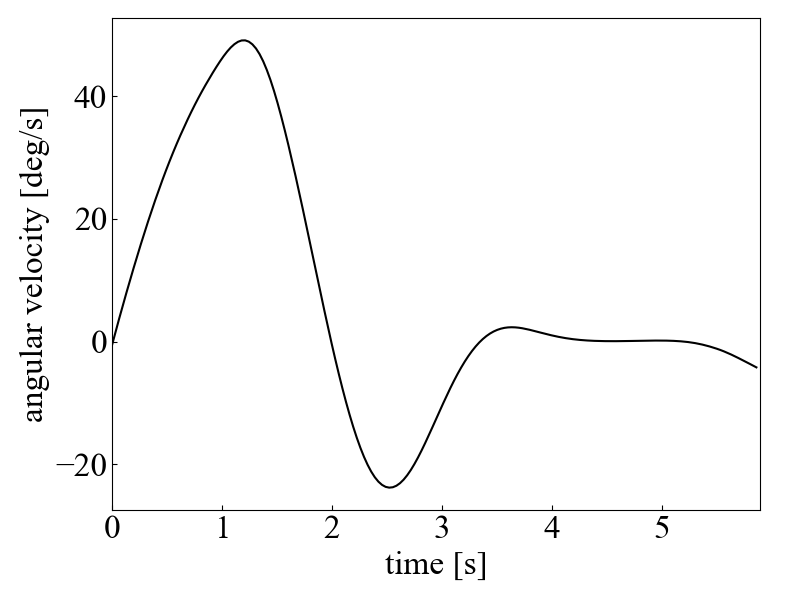
\includegraphics[width=\columnwidth]{./figure/crossdegpers.png}
	  \caption{B-dot制御の角速度推移}
	  \label{fig:crossdegpers}
	\end{minipage}
\end{figure}


\subsection{考察}
 各結果の整定時間,定常偏差を表\ref{table:result}に示す.
この表から,整定時間に基づいて評価すればB-dot制御則が最適であり,
定常偏差に基づいて評価すればクロスプロダクト則が最も優れた制御則となる結果を得た.

\begin{table}[H]
	\centering
	\caption{実験結果}
	\label{table:result}
	\begin{tabular}{|c||c|c|c|c|c|c|}
		\hline
		 & 50\% & 100\% & P制御 & PD制御 & B-dot制御則 & クロスプロダクト制御則 \\ \hline
		整定時間T [s] & 4.1 & 4.3 & 3.8 & 4.0 & 3.0 & 3.8 \\ \hline
		定常偏差$\theta$ [deg] & 0 & 0 & 2.78 & -21.3 & -13.4 & 0.1 \\ \hline
	\end{tabular}
\end{table}


\newpage
\section{結論}
\subsection{本研究のまとめ}
 本研究では,人工衛星の模型や実験システムを新規に作製して,磁気トルカによる姿勢制御を検証した.

先行研究では,想定される人工衛星の大きさの違いや,磁気トルカでの検証を行われていなかったため,超小型人工衛星の,特に磁気トルカに注目して実験装置を作製し,検証を行った.定常偏差を無視すればB-dot制御則が,定常偏差を考慮すればクロスプロダクト則が最も性能の良い制御理論となる結果を得た.

摩擦の影響がない宇宙空間を想定すると,積分要素が含まれていなくても定常偏差は残らない.転がり軸受の工夫等により摩擦をさらに軽減できれば,PD制御・クロスプロダクト則は定常偏差が残らず,B-dot制御則との役割の違いが現れ,評価が変わる可能性がある. 

今回は磁気トルカを1本のみ用いて検証を行った.しかし実際の人工衛星の姿勢制御では,1軸に対して磁気トルカを2本用いて姿勢制御を行っていることも多いため,磁気トルカをもう1本増やした検証も必要であると考える.

\subsection{今後の展望}

 摩擦の影響がない宇宙空間を想定すると,積分要素が含まれていなくても定常偏差は残らない.転がり軸受の工夫等により摩擦をさらに軽減できれば,PD制御・クロスプロダクト則は定常偏差が残らず,B-dot制御則との役割の違いが現れ,評価が変わる可能性がある. 

今回は磁気トルカを1本のみ用いて検証を行った.しかし実際の人工衛星の姿勢制御では,1軸に対して磁気トルカを2本用いて姿勢制御を行っていることも多いため,磁気トルカをもう1本増やした検証も必要であると考える.

また,作製した模型の